%-*- coding: utf-8 -*-
\subsection{Génération automatique des menus}
\begin{figure}[H]
\label{MenuGen}
  \centering
      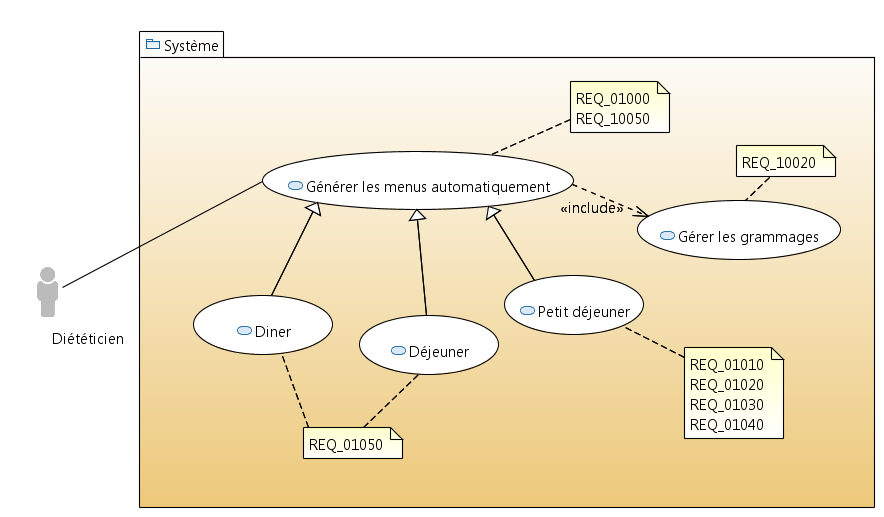
\includegraphics[width=1.00\textwidth]{../../CasDUtilisations/MenuGen/MenuGen.png} %
\caption{Génération automatique des menus}
\end{figure}

\begin{description}
\item[Nom:] Génération automatique des menus.
\item[ID:] UC103
\item[Description:] Permet la génération automatique des menus.
\item[Auteur:] Jean-Félix BENITEZ.
\item[Date:] 07/05/2017
\item[Acteurs:] Diététiciens.
\item[Pré-Conditions:] Le diététicien s'est connecté au système.
\item[Scénario principal:]
  \begin{enumerate}
  \item Le diététicien sélectionne le groupe de patients pour lequel il veut générer les menus,
  \item ensuite il lance la génération automatique.
  \item la génération automatique ce déroule en prenant en compte les grammages.
  \end{enumerate}
\item[Scénario alternatif:] Aucun.
\item[Post-Conditions:] Les menus sont générés.
\end{description}
